% =====================================================================
\chapter{Ajuste supervisado con instrucciones}
\label{tema:2}
% =====================================================================

Este tema define el ajuste supervisado (SFT, del inglés \emph{supervised fine-tuning}) de un modelo de lenguaje: la misma entropía cruzada del preentrenamiento, evaluada solo en las posiciones de la respuesta. Se estudian los datos de instrucciones, la pérdida enmascarada y su interpretación probabilística, los detalles de construcción de lotes y la plantilla de chat. Se sigue el §8.1 de Jurafsky y Martin~\cite{jm3}, la clase~15 de CS336~\cite{cs336} y su tarea~5~\cite[§4.2]{cs336a5}, y los artículos de FLAN~\cite{wei-flan}, T0~\cite{sanh-t0}, InstructGPT~\cite[§3.2 y~§3.5]{ouyang} y LIMA~\cite{zhou-lima}.

\section{Datos de instrucciones}

\begin{definicion}[Conjunto de instrucciones]\label{def:instrucciones}
Un \emph{conjunto de instrucciones} es una colección de pares $\{(u^{(i)},y^{(i)})\}_{i=1}^{n}$ en la que $u^{(i)}$ es una instrucción en lenguaje natural, que puede incluir un texto de entrada, e $y^{(i)}$ es la respuesta deseada. El \emph{ajuste con instrucciones} (\emph{instruction tuning}) es el ajuste supervisado sobre un conjunto de instrucciones que abarca muchas tareas distintas.
\end{definicion}

Los conjuntos se construyen de dos maneras~\cite[§8.1.1]{jm3}: reformulando como instrucciones conjuntos de datos supervisados ya existentes, mediante plantillas, o recogiendo demostraciones escritas por personas (o generadas por otros modelos). La colección Flan 2022, por ejemplo, reúne 15 millones de ejemplos de 1836 tareas~\cite[§8.1.1]{jm3}.

\begin{definicion}[Generalización a tareas no vistas]\label{def:no-vistas}
Se agrupan las tareas en \emph{grupos} (traducción, resumen, inferencia, preguntas y respuestas, etc.). Para medir la generalización a tareas no vistas se ajusta el modelo con todos los grupos salvo uno y se evalúa sin ejemplos (\emph{zero-shot}) en las tareas del grupo excluido.
\end{definicion}

Con este protocolo, Wei \emph{et al.}~\cite{wei-flan} ajustaron un modelo de 137\,000 millones de parámetros con más de 60 conjuntos de datos expresados mediante plantillas de instrucciones (FLAN). El modelo ajustado superó, sin ejemplos, a GPT-3 de 175\,000 millones de parámetros en 20 de los 25 conjuntos evaluados, y el beneficio dependía de la escala: en los modelos más pequeños estudiados, el ajuste con instrucciones empeoraba el resultado en las tareas no vistas. Sanh \emph{et al.}~\cite{sanh-t0} obtuvieron resultados análogos con T0, un modelo de tipo T5 de 11\,000 millones de parámetros ajustado con una colección de conjuntos de datos reformulados mediante múltiples \emph{prompts}, que igualaba o superaba en varias pruebas a modelos hasta 16 veces mayores.

\begin{observacion}[El ajuste supervisado en InstructGPT]\label{obs:instructgpt}
En InstructGPT~\cite{ouyang}, el primer paso usa unas 13\,000 instrucciones de entrenamiento con demostraciones escritas por anotadores~\cite[§3.2]{ouyang}. El modelo se ajusta durante 16 épocas con decaimiento coseno de la tasa de aprendizaje y \emph{dropout} residual de $0{,}2$; la pérdida de validación empieza a subir después de la primera época, pero entrenar más épocas mejora la puntuación del modelo de recompensa y las preferencias humanas~\cite[§3.5]{ouyang}. La pérdida de validación del SFT no es, por tanto, un indicador fiable de la calidad final.
\end{observacion}

\section{La pérdida enmascarada}

Sean $u=u_{1:n}$ la instrucción e $y=y_{1:m}$ la respuesta, ambas ya tokenizadas, y sea $x_{1:T}=(u_1,\dots,u_n,y_1,\dots,y_m)$, con $T=n+m$, la secuencia concatenada. El último token de $y$ es el token de fin de turno.

\begin{definicion}[Pérdida del ajuste supervisado]\label{def:sft}
Sea $m_t\in\{0,1\}$ una \emph{máscara} que vale $1$ en las posiciones de la respuesta ($t>n$) y $0$ en las de la instrucción. La \emph{pérdida del ajuste supervisado} es la entropía cruzada enmascarada
\[
\Lsft(\theta)=-\frac{1}{\sum_{t=1}^{T}m_t}\sum_{t=1}^{T}m_t\ln p_\theta(x_t\mid x_{1:t-1}).
\]
\end{definicion}

Se divide por el número de posiciones que cuentan, no por $T$. Si $m_t=1$ para todo $t$, se recupera la pérdida del preentrenamiento.

\begin{proposicion}[Interpretación probabilística]\label{prop:sft-condicional}
Con la máscara de la \cref{def:sft},
\[
\Lsft(\theta)=-\frac{1}{m}\ln p_\theta(y\mid u),\qquad\text{donde}\quad p_\theta(y\mid u)=\prod_{j=1}^{m}p_\theta(y_j\mid u,y_{1:j-1}).
\]
En consecuencia, minimizar la suma de $m^{(i)}\Lsft^{(i)}$ sobre un conjunto de instrucciones equivale a estimar por máxima verosimilitud la distribución condicional de la respuesta dada la instrucción.
\end{proposicion}

\begin{proof}
Como $m_t=0$ para $t\le n$ y $m_t=1$ para $t=n+j$, $j=1,\dots,m$, se tiene $\sum_t m_t=m$ y
\[
\sum_{t=1}^{T}m_t\ln p_\theta(x_t\mid x_{1:t-1})=\sum_{j=1}^{m}\ln p_\theta(y_j\mid u,y_{1:j-1})=\ln\prod_{j=1}^{m}p_\theta(y_j\mid u,y_{1:j-1}).
\]
Por la regla de la cadena (módulo~1, tema~2) aplicada a la distribución condicionada a $u$, el producto es $p_\theta(y\mid u)$. Dividiendo por $m$ y cambiando el signo se obtiene la igualdad. La suma $\sum_i m^{(i)}\Lsft^{(i)}=-\sum_i\ln p_\theta(y^{(i)}\mid u^{(i)})$ es la log-verosimilitud negativa condicional del conjunto.
\end{proof}

\begin{observacion}
Sin máscara se minimizaría $-\frac{1}{T}\ln p_\theta(u,y)=-\frac1T\bigl(\ln p_\theta(u)+\ln p_\theta(y\mid u)\bigr)$: el modelo dedicaría parte de su capacidad a imitar las instrucciones de los usuarios, que no tiene que generar. Este es el sentido de la indicación de Jurafsky y Martin de entrenar solo sobre la respuesta~\cite[§8.1]{jm3}.
\end{observacion}

\begin{proposicion}[Gradiente en las posiciones enmascaradas]\label{prop:grad-mascara}
Sea $z_t\in\R^{K}$ el vector de logits de la posición $t$ y $p_t=\softmax(z_t)$. Entonces
\[
\frac{\partial\Lsft}{\partial z_t}=\frac{m_t}{\sum_{s}m_s}\,\bigl(p_t-e_{x_t}\bigr),
\]
donde $e_{x_t}$ es el vector canónico del token objetivo. En particular, el gradiente respecto a los logits de una posición enmascarada es nulo.
\end{proposicion}

\begin{proof}
Solo el sumando $t$ depende de $z_t$. Como $-\ln p_\theta(x_t\mid x_{1:t-1})=\LSE(z_t)-(z_t)_{x_t}$ y $\nabla\LSE(z)=\softmax(z)$ (módulo~1, tema~4), su gradiente es $p_t-e_{x_t}$. Basta multiplicar por el coeficiente $m_t/\sum_s m_s$.
\end{proof}

\begin{observacion}
Que el gradiente respecto a los logits de la instrucción sea nulo no implica que la instrucción no influya en el aprendizaje: las posiciones de la respuesta atienden a las de la instrucción, de modo que el gradiente llega a los estados ocultos de la instrucción a través de la atención. Lo que se suprime es la señal que obligaría a \emph{predecir} los tokens de la instrucción.
\end{observacion}

\begin{ejemplo}[Con máscara y sin ella]\label{ej:mascara}
Una secuencia tiene 4 tokens de instrucción y 2 de respuesta, con pérdidas por token $-\ln p$ de $2{,}0$; $1{,}5$; $0{,}5$; $1{,}0$ en la instrucción y $0{,}4$; $0{,}2$ en la respuesta. Sin máscara, la pérdida es $(2{,}0+1{,}5+0{,}5+1{,}0+0{,}4+0{,}2)/6=5{,}6/6=0{,}933$; con máscara, $(0{,}4+0{,}2)/2=0{,}300$. En la práctica del módulo, la muestra «p: doble de 2\textbackslash n r: 4» tiene 18 posiciones de predicción, de las que solo 3 puntúan (el espacio, «4» y el token de fin): un $16{,}7\,\%$.
\end{ejemplo}

\begin{observacion}[Implementación]
En PyTorch no se multiplica por la máscara de forma explícita: se asigna la etiqueta $-100$ a las posiciones que no cuentan y la función \texttt{cross\_\allowbreak entropy} con \texttt{ignore\_index=-100}, el valor por defecto, las excluye del numerador y del denominador de la media.
\end{observacion}

\section{Lotes: relleno, normalización, empaquetado y acumulación}

Las secuencias de un lote tienen longitudes distintas. Hay dos formas de formar tensores rectangulares.

\begin{definicion}[Relleno y empaquetado]\label{def:relleno}
En el \emph{relleno} (\emph{padding}) cada secuencia se completa con un token de relleno hasta la longitud máxima del lote, y la máscara vale $0$ en las posiciones de relleno. En el \emph{empaquetado} (\emph{packing}) se concatenan los ejemplos, separados por el token de fin, y la cadena resultante se corta en trozos consecutivos de longitud fija $L$.
\end{definicion}

El empaquetado no desperdicia posiciones, pero un trozo puede contener el final de un ejemplo y el principio de otro; la máscara causal permite entonces que un ejemplo atienda al anterior, lo que suele tolerarse porque el token de fin los separa.

Sea un lote de $B$ secuencias con máscaras $m^{(i)}_t$ y pérdidas por token $\ell^{(i)}_t=-\ln p_\theta(x^{(i)}_t\mid x^{(i)}_{1:t-1})$, y sea $M_i=\sum_t m^{(i)}_t$. Hay dos normalizaciones habituales:
\[
J_{\mathrm{tok}}=\frac{\sum_{i}\sum_t m^{(i)}_t\ell^{(i)}_t}{\sum_i M_i},\qquad
J_{\mathrm{sec}}=\frac{1}{B}\sum_{i=1}^{B}\frac{1}{c}\sum_t m^{(i)}_t\ell^{(i)}_t,
\]
con $c>0$ una constante fija (por ejemplo, la longitud máxima). En $J_{\mathrm{tok}}$ cada secuencia pesa en proporción a la longitud de su respuesta; en $J_{\mathrm{sec}}$ todas las secuencias pesan lo mismo por cada token, independientemente del lote en el que caigan. La tarea~5 de CS336 implementa una normalización del segundo tipo: una suma enmascarada dividida por una constante~\cite[§4.2]{cs336a5}.

\begin{proposicion}[Acumulación de gradientes]\label{prop:acumulacion}
Divídase un lote de $B$ secuencias en $G$ microlotes $\mathcal{B}_1,\dots,\mathcal{B}_G$ de $B/G$ secuencias. Sea $J_g$ la pérdida $J_{\mathrm{sec}}$ del microlote $g$ calculada con tamaño $B/G$. Si cada microlote retropropaga $J_g/G$ y se suman los gradientes antes de actualizar, el gradiente acumulado coincide con el de $J_{\mathrm{sec}}$ sobre el lote completo.
\end{proposicion}

\begin{proof}
Sea $S_i=\frac1c\sum_t m^{(i)}_t\ell^{(i)}_t$. Entonces $J_g=\frac{G}{B}\sum_{i\in\mathcal{B}_g}S_i$ y
\[
\sum_{g=1}^{G}\frac{J_g}{G}=\sum_{g=1}^{G}\frac{1}{B}\sum_{i\in\mathcal{B}_g}S_i=\frac{1}{B}\sum_{i=1}^{B}S_i=J_{\mathrm{sec}},
\]
porque los microlotes forman una partición del lote. Por la linealidad del gradiente, $\sum_g\nabla(J_g/G)=\nabla J_{\mathrm{sec}}$.
\end{proof}

\begin{observacion}
Con la normalización $J_{\mathrm{tok}}$ la equivalencia falla en general: cada microlote divide por su propio número de tokens de respuesta y la suma de los cocientes no es el cociente de las sumas, salvo que todos los microlotes tengan el mismo número de tokens que puntúan.
\end{observacion}

\section{La plantilla de chat}

Un diálogo es una lista de mensajes $(r_1,c_1)$, \dots, $(r_J,c_J)$, donde $r_j\in\{\text{sistema},\text{usuario},\text{asistente}\}$ es el rol y $c_j$ el contenido. Para tratarlo con un modelo autorregresivo hay que convertirlo en una única secuencia.

\begin{definicion}[Plantilla de chat]\label{def:plantilla}
Sea $\V$ un vocabulario ampliado con un token especial por rol, $\langle r\rangle$, y un token de fin de turno, $\langle\mathrm{fin}\rangle$, que no aparecen en el texto ordinario. La \emph{plantilla de chat} asigna al diálogo la secuencia
\[
\langle r_1\rangle\,\tau(c_1)\,\langle\mathrm{fin}\rangle\ \langle r_2\rangle\,\tau(c_2)\,\langle\mathrm{fin}\rangle\ \cdots\ \langle r_J\rangle\,\tau(c_J)\,\langle\mathrm{fin}\rangle,
\]
donde $\tau$ es el tokenizador. En el ajuste supervisado, la máscara vale $1$ en los tokens de $\tau(c_j)$ y en el $\langle\mathrm{fin}\rangle$ que los cierra si $r_j=\text{asistente}$, y $0$ en el resto.
\end{definicion}

\begin{figure}[h]
\centering
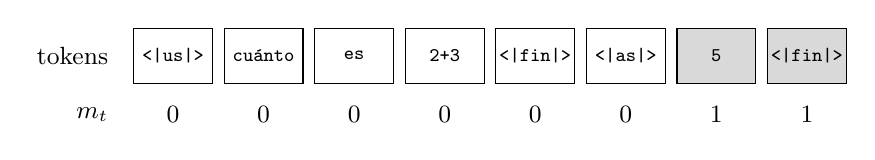
\begin{tikzpicture}[font=\small,
  t/.style={draw,minimum height=7mm,minimum width=10mm,inner sep=1pt,font=\scriptsize\ttfamily},
  on/.style={t,fill=black!15}]
  \foreach \txt/\st [count=\i] in {<|us|>/t,cuánto/t,es/t,2+3/t,<|fin|>/t,<|as|>/t,5/on,<|fin|>/on}{
    \node[\st] (n\i) at (1.15*\i,0) {\txt};
  }
  \foreach \v [count=\i] in {0,0,0,0,0,0,1,1}{
    \node[font=\small] at (1.15*\i,-0.75) {$\v$};
  }
  \node[anchor=east,font=\small] at (0.45,0) {tokens};
  \node[anchor=east,font=\small] at (0.45,-0.75) {$m_t$};
\end{tikzpicture}
\caption{Plantilla de chat de un turno (\texttt{us}: usuario; \texttt{as}: asistente) y su máscara. Solo puntúan el contenido de la respuesta y el token de fin que la cierra (sombreados).}
\label{fig:plantilla}
\end{figure}

En la inferencia, la aplicación construye la plantilla con todo el historial, añade $\langle\text{asistente}\rangle$ y deja que el modelo genere hasta emitir $\langle\mathrm{fin}\rangle$. Incluir el token de fin en la pérdida es imprescindible para que el modelo aprenda a terminar su turno: en la práctica del módulo, el modelo base no lo emite nunca y, tras 600 pasos de SFT, lo emite en el $99{,}4\,\%$ de los ejemplos de entrenamiento y en el $100\,\%$ de los de prueba.

\begin{observacion}
Los tokens especiales se añaden al vocabulario antes del ajuste (módulo~12) y sus vectores de \emph{embedding} se aprenden durante él. Por eso la plantilla forma parte del modelo: usar un modelo ajustado con una plantilla distinta de la suya degrada su comportamiento. Cada laboratorio usa su propio formato interno y no siempre lo publica; lo que documentan públicamente las API de Claude, Gemini y Grok es que los mensajes se envían como una lista de pares (rol, contenido).
\end{observacion}

\section{¿Cuántos datos hacen falta? La alineación superficial}

El preentrenamiento consume billones de tokens; el ajuste supervisado publicado usa entre miles y cientos de miles de diálogos. Zhou \emph{et al.}~\cite{zhou-lima} ajustaron un modelo LLaMa de 65\,000 millones de parámetros con solo 1000 pares instrucción--respuesta seleccionados con cuidado (LIMA); en una evaluación humana controlada, sus respuestas empataron con las de GPT-4 o fueron preferidas a ellas en el $43\,\%$ de los casos. De ahí la \emph{hipótesis de la alineación superficial}: casi todo el conocimiento del modelo se adquiere en el preentrenamiento, y el ajuste enseña sobre todo qué formato y qué estilo usar al interactuar con un usuario. En la misma línea, Dettmers \emph{et al.}~\cite[§1]{dettmers} observaron que un conjunto de 9000 diálogos de alta calidad (OASST1) daba mejores asistentes que una submuestra de 450\,000 ejemplos de FLAN~v2.

\begin{observacion}
Estas conclusiones proceden de evaluaciones concretas de calidad conversacional y no implican que los datos de SFT sean irrelevantes para todas las capacidades: tareas como el razonamiento matemático o la programación se benefician de muchos más ejemplos. La lección robusta es que la calidad y la diversidad de los datos pesan más que su cantidad.
\end{observacion}

\begin{lecturas}
\item Jurafsky y Martin~\cite{jm3}, §8.1 «Instruction Tuning», con §8.1.1 (datos) y §8.1.2 (evaluación).
\item CS336~\cite{cs336}, clase~15 «Alignment -- SFT/RLHF», y tarea~5~\cite[§4]{cs336a5}.
\item CS224N~\cite{cs224n}, clase~8 «Post-training».
\item Wei \emph{et al.}~\cite{wei-flan} (FLAN) y Sanh \emph{et al.}~\cite{sanh-t0} (T0).
\item Ouyang \emph{et al.}~\cite{ouyang}, §3.2 (datos) y §3.5 (modelos), y Zhou \emph{et al.}~\cite{zhou-lima}.
\end{lecturas}

\section*{Ejercicios del tema 2}
\addcontentsline{toc}{section}{Ejercicios del tema 2}

\begin{ejercicio}{1}{eje:2-base}
Explique por qué un modelo base, al recibir «p: capital de francia\textbackslash n r:», no responde «paris» aunque el dato esté en su texto de entrenamiento, y qué le enseña el ajuste supervisado.
\end{ejercicio}

\begin{ejercicio}{1}{eje:2-ignore}
¿Qué ocurre con una posición cuya etiqueta vale $-100$ en \texttt{cross\_entropy(\dots, ignore\_index=-100)}? ¿Por qué se usa también en las posiciones de relleno?
\end{ejercicio}

\begin{ejercicio}{2}{eje:2-mascara}
Una secuencia tiene 4 tokens de instrucción con pérdidas $2{,}1$; $1{,}8$; $0{,}9$; $1{,}1$ y 3 de respuesta con $0{,}6$; $0{,}2$; $0{,}4$. Calcule la pérdida media sin máscara y con máscara.
\end{ejercicio}

\begin{ejercicio}{1}{eje:2-tokenizar}
Se tienen dos ejemplos tokenizados. Ejemplo~1: instrucción $[5,9,2]$ y respuesta $[7,3,0]$. Ejemplo~2: instrucción $[4,8]$ y respuesta $[6,0]$. El índice~0 es el token de fin y el~1, el de relleno. Concatene instrucción y respuesta, rellene a la longitud máxima y construya \texttt{input\_\allowbreak ids} (la secuencia sin su último token), \texttt{labels} (la secuencia sin su primer token) y \texttt{response\_\allowbreak mask} (1 donde la etiqueta pertenece a la respuesta). ¿Cuántas posiciones puntúan en cada ejemplo?
\fuente{adaptado de Stanford CS336, primavera de 2025, tarea~5~\cite[§4.2]{cs336a5}, problema \texttt{tokenize\_\allowbreak prompt\_\allowbreak and\_\allowbreak output}.}
\end{ejercicio}

\begin{ejercicio}{2}{eje:2-microlote}
Un microlote tiene 2 secuencias de 5 posiciones, con log-probabilidades por token $(-2{,}0;\,-1{,}5;\,-0{,}5;\,-1{,}0;\,-0{,}1)$ y $(-1{,}2;\,-0{,}4;\,-0{,}2;\,-3{,}0;\,-3{,}0)$ y máscaras de respuesta $(0,0,1,1,1)$ y $(0,1,1,0,0)$. La pérdida del microlote es la suma enmascarada de $-\ln p$ dividida por el tamaño del microlote, por una constante $c=1$ y por el número de pasos de acumulación, $2$. Calcule esa pérdida y compárela con la media por token de respuesta, $J_{\mathrm{tok}}$.
\fuente{adaptado de Stanford CS336, primavera de 2025, tarea~5~\cite[§4.2]{cs336a5}, problemas \texttt{masked\_\allowbreak normalize} y \texttt{sft\_\allowbreak microbatch\_\allowbreak train\_\allowbreak step}.}
\end{ejercicio}

\begin{ejercicio}{1}{eje:2-empaquetar}
Se tienen tres ejemplos de 7, 5 y 9 tokens. Se añade un token de fin tras cada uno, se concatenan y se corta la cadena en trozos consecutivos de 5 tokens, descartando el último si está incompleto. ¿Cuántas secuencias se obtienen y cuántos tokens se pierden? Compárese con rellenar cada ejemplo, con su fin, hasta 10 tokens: ¿qué fracción de posiciones es útil en cada caso?
\fuente{adaptado de Stanford CS336, primavera de 2026, suplemento de la tarea~5~\cite[§4.2]{cs336a5s}, problema \texttt{data\_\allowbreak loading}.}
\end{ejercicio}

\begin{ejercicio}{3}{eje:2-multiturno}
Un diálogo alterna $K$ turnos de usuario $u^{(1)},\dots,u^{(K)}$ y $K$ respuestas del asistente $y^{(1)},\dots,y^{(K)}$, de longitudes $m_1,\dots,m_K$, en el orden $u^{(1)},y^{(1)},\dots,u^{(K)},y^{(K)}$. Con la máscara de la \cref{def:plantilla}, demuestre que
\[
\Lsft=-\frac{1}{\sum_k m_k}\sum_{k=1}^{K}\ln p_\theta\bigl(y^{(k)}\,\big|\,h^{(k)}\bigr),
\]
donde $h^{(k)}=(u^{(1)},y^{(1)},\dots,u^{(k)})$ es el historial que precede a la respuesta $k$ (se omiten los tokens de rol y de fin para simplificar). Interprete el resultado.
\end{ejercicio}
